\section{Introduction}
\label{sec:intro}
The CMS Collaboration recently published a search for new physics
in events with same-sign isolated dileptons, jets, and \met~\cite{sspaper}. In that study the major
background is from \ttbar production, as shown in Fig.~\ref{fig:ttbar}.

\begin{figure}[htb]
\begin{center}
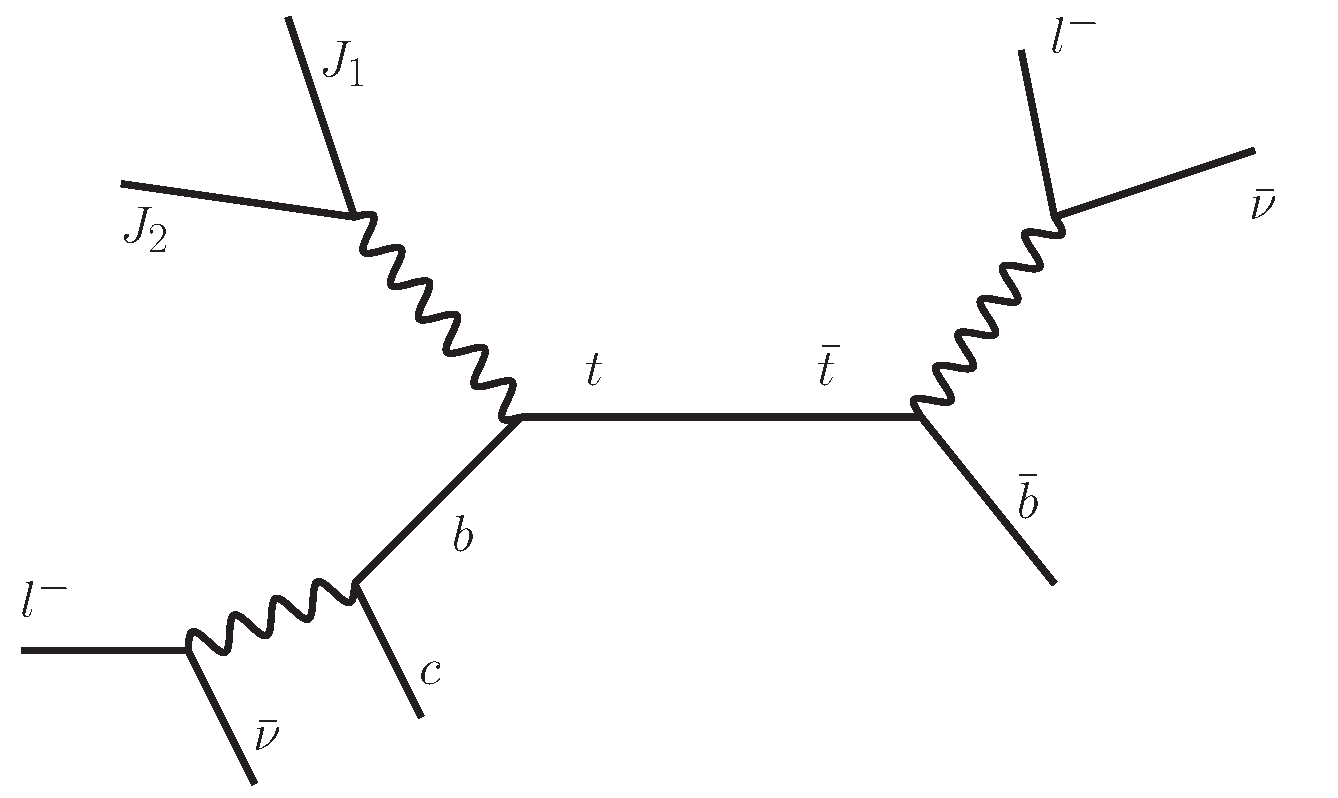
\includegraphics[width=0.6\linewidth, height=0.35\linewidth]{figs/ttbar.pdf}
\caption{ Diagram for \ttbar decays giving rise to same-sign dilepton final states \label{fig:ttbar}}
\end{center}
\end{figure}

The dominant source of same-sign dileptons in \ttbar events are produced via, $t \rightarrow W b$; where 
one of the leptons is from $W \rightarrow \ell \nu $ and the other originates from semi-leptonic $b$ decays. 
An additional requirement on the number of $b$ jets $\geq 2$, is expected to reduce this background significantly
as a b-quark can not produce an isolated lepton and at the same time provide a b-tag.

In this note we perform an inclusive search for new physics  in events with two isolated, same-sign dileptons,
in association with at least 2 $b$ jets and \met. This generic signature should also be sensitive to SUSY involving
third generation fermions.  For the purpose of this note we restrict ourselves to the $ee$, $e\mu$, and $\mu\mu$ 
final states, {\em i.e.}, we do not consider $\tau$'s, except in the case that the $\tau$ decays leptonically.

This note is organized as follows: in Section~\ref{searchbtag} we briefly outline the event selection used in this study 
along with event yields and backgound estimation as well as a discussion on the background. The description of systematics uncertanities on the 
acceptance is given in Section~\ref{systematic}.  Finally, in Section~\ref{sec:ssresults} we summarize the results followed by 
the conclusion in Section~\ref{sec:conclusion}.




